\documentclass{article}
\usepackage[utf8]{inputenc}
\usepackage[spanish]{babel}
\usepackage{listings}
\usepackage{graphicx}
\graphicspath{ {/home/mafeta/Imágenes/parcial1}}
\usepackage{cite}

\begin{document}

\begin{titlepage}
    \begin{center}
        \vspace*{1cm}
            
        \Huge
        \textbf{Implementación Parcial 1}
            
        \vspace{0.5cm}
        \LARGE
        Sistema de desencriptación 
            
        \vspace{5cm}
            
        \textbf{Maria Fernanda Tasco ALquichire}
            
        \vfill
            
        \vspace{0.8cm}
            
        \Large
        Despartamento de Ingeniería Electrónica y Telecomunicaciones\\
        Universidad de Antioquia\\
        Medellín\\
        Febrero de 2022
            
    \end{center}
\end{titlepage}

\tableofcontents
\newpage

\section{Objetivos}\label{intro1}
\subsection{generales}
resumen - abstrac
\subsection{Especificos}
introducion

\section{Sección introductoria}\label{intro2}
\subsection{Resumen}
resumen - abstrac
\subsection{Introdución}
introducion

\section{Sección introductoria}\label{investigación}


\section{Aplicación en tinkercad}\label{practica}
En el proyecto de  \textbf{tinkercad } \cite{implementacion} se tuvo en cuenta estos aspectos:
\begin{flushleft}
    • se tuvo en cuenta estos aspectos del integrado\\[0.1cm]
        
        ◦ Su función de desplazamiento que permitó manejar la entrada bit a bit y tener más control de ello \\[0.1cm]
        ◦ Que la salida fuera en paralelo permitió la manipulación de bits de manera individual para poder compararlos. \\[0.1cm]
        
    • se uso estos integrados para el sistema de comparación.\\[0.1cm]
        ◦ Una compuerta XOR  la cual ayudaría a que según su logica la salida fuera 0/bajo si los bits de comparación eran iguales. Se uso dos integrados 74hc86 ya que tiene 4 compuertas lógicas XOR y se necesitaba 8 para la compración de los 8 bits\\[0.1cm]
        ◦ Las salidas de las compuertas XOR van a las entradas de las compuertas NOT para que así su valor fuera más fácil de representar con un 1 que un 0 cuando los bits fueran iguales. Se uso 2 CI 74hc04, debido a que este tiene 6 compuertas not y se necesitaban 8 para negar cada salida.\\[0.1cm]
         ◦ Para que al final tuviera una sola salida se uso compuertas AND que iban comparando las salidas de estos NOT. Se uso 2 CI74hc08 ya que se necesitaban 7 compuertas AND\\[0.1cm]
    Aquí en la figura 1 un ejemplo del diagrama que se uso para un entendimiento y organización más sencilla a la hora de implementarlo.
    
    \begin{figure}[!ht]
    \caption{Implementación sistema de compración el Logicsim}
    \centering
    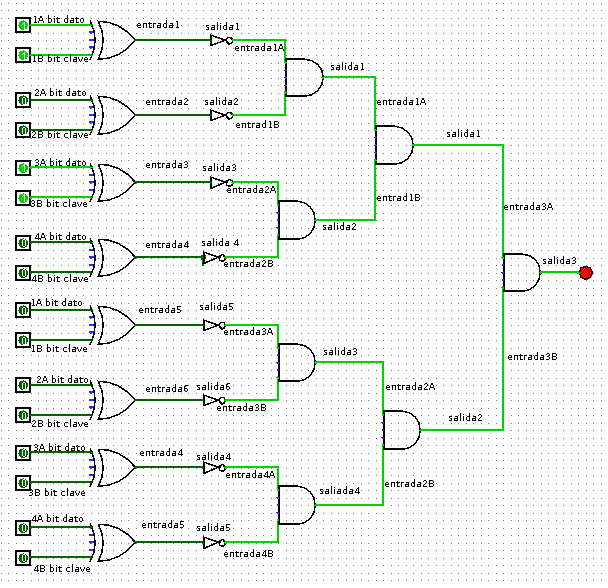
\includegraphics[width=0.5\textwidth]{sistema_compracion_pines.png}
    \end{figure}
    
    • Para llegar a una solución se decidió hacer una prueba de escritorio la cuál tuvo en cuenta los siguentes aspectos: \\[0.1cm]
        ◦ Pasar el arreglo desde el arduino esclavo al arduino maestro. Se descarto este idea por el tiempo que toma pasar datos de gran magnitud.\\[0.1cm]
        ◦ El arreglo lo van a tener inicialmente los dos arduinos. Con la idea de que el arduino esclavo le mande la información al 74hc595 se haga el sistema de desencriptación y luego se mande la señal de compración y ya sea bajo/alta el arduino maestro irá recorriendo el arreglo original, así cuando se mande una señal alta este tenga la posición de la clave y pueda moverse desde allí para sacar el mensaje real.\\[0.1cm]
         ◦ El mensaje real será guardado poir el arduino maestro en un arreglo para luego ser mostrado en la lcd\\[0.1cm]
         ◦ Se decidió no pasar ningún dato por los arduinos ya que al ser un sistema de encriptación no sería buena en transferir datos o señales directamente entre ellos.[0.1cm]
    • Se decidió usar la función Shiftout para el desplazamiento y mandar las señales de reloj al integrado 74hc595. \\[0.1cm]
\end{flushleft}





(\ref{intro1}),(\label{intro2}), (\label{investigación}) y  (\label{practica})
\bibliographystyle{IEEEtran}
\bibliography{references}

\end{document}

https://forum.arduino.cc/t/contador-con-74hc595-display-7-segmentos-solucionado/640032
https://drive.google.com/file/d/1BAaL1Y0o128aGsjOiQicpK0ooIhtqbEt/view

para el pc1 que genera los datos  https://www.cplusplus.com/reference/ostream/ostream/write/